\section{Problem Formulations, Scores \& Evaluation Metrics}

In this project, we address the task of temporal action segmentation in professional bouldering videos. The objective is to classify each frame of a video based on the climber's activity.

\subsection{Video Representation}
We represent each video as a sequence of frames $video_i = \{f_1, f_2, \cdots, f_N\}$ where $f_i$ is a frame represented by a tensor of size $C \times H \times W$, with $C$ being the number of channels (fixed to 3 for RGB videos), $H$ the video height, $W$ the video width, and $N$ the total number of frames in the video.

The video's duration (in seconds) can be calculated as $\text{Duration} = \frac{N}{F}$ where $F$ is the video's frame rate which will be fixed to $25$ during our experiments.

\subsection{Annotation Representation}
Each video's annotations are provided at the frame level. Given a video $video_i$, its corresponding annotations are defined as $a_i = \{c_1, c_2, \cdots, c_N\}$ where $c_i \in C$, and $C$ is the set of all possible activity labels. In our case $C = \{\text{Observing}, \: \text{Brushing}, \: \text{Cleaning}, \: \text{Stopwatch} \}$

\subsection{Problem Formulation}
The goal is to develop a model $f$ that takes a video as input and predicts the corresponding sequence of frame-level annotations $f : video_i \rightarrow a_i$. Alternatively, the model can be designed to:

\quad \emph{1. Frame-wise Prediction:} The model processes each frame independently and predicts its corresponding label:  
    $f_{frame} : f_t \rightarrow c_t$.

\quad \emph{2. Sequence-based Prediction:} The model processes a sequence of $T$ frames and predicts a single label for the entire sequence:  
    $f_{seq} : \{f_{t}, f_{t+1}, \cdots, f_{t+T-1} \} \rightarrow c_t$.

The choice between these formulations may depend on the desired balance between temporal context awareness and computational efficiency.

% As specified during the previous section we are dealing with videos and their annotations.

% We are going to represent videos as a sequence of frames $Video_i = \{f_1, f_2, \cdots, f_N\}$ where $f_i$ is a frame which is represented by a tensor of size C, H, W with C the number of channels that is fixed to 3, H the video height and W the width and $N$ the number of frames in the video and $F$ the frame rate of the video.
% The video duration in seconds can be retrieved by doing $\frac{N}{F}$ seconds. 

% The annotations of a video will also be represented in a frame level, give a $Video_i$, its corresponding annotations $A_i = \{c_1, c_2, \cdots, c_N\}$ with $c_i \in C$ where $C$ is the set of all possible classes \ labels in the video, in our case $C = \{ \text{Observing}, \: \text{Brushing}, \: \text{Cleaning}, \: \text{Stopwatch} \}$.

% Given this the idea is to develop a model $f$ that will be given a video and produce annotations for each frame of it. We can also imagine that the model can take in a single frame and produce a single annotations for the corresponding frame, or take in sequence of T frames and produce a single annotations for the sequence.

% Read other papers and see how they formulate the problem.


\subsection{Problem Formulations}

Here we give the notations, formulations, etc that will be used throughout the project.

We give the TAS formulation of the problem and cite the TAS review paper.

And we also present different equivalent formulations of the problem.

Each formulation and notation must be explained with an illustration, we'll be using a four column illustration in order to not take up too much space.

Finally we end up by referring to the notation that we opted to use.

\begin{figure*}[h]
    \centering
    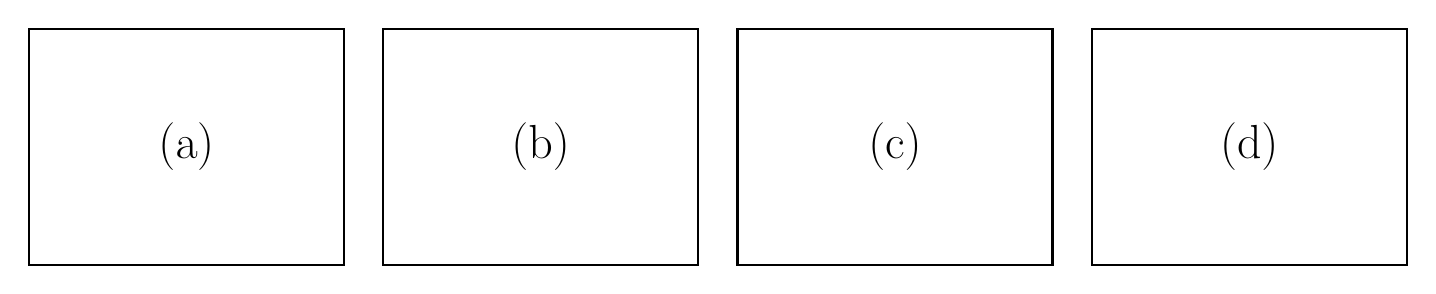
\begin{tikzpicture}
        % First column
        \draw[thick] (0,0) rectangle (4,3);
        \node at (2,1.5) {\LARGE (a)};

        % Second column
        \draw[thick] (4.5,0) rectangle (8.5,3);
        \node at (6.5,1.5) {\LARGE (b)};

        % Third column
        \draw[thick] (9,0) rectangle (13,3);
        \node at (11,1.5) {\LARGE (c)};

        % Fourth column
        \draw[thick] (13.5,0) rectangle (17.5,3);
        \node at (15.5,1.5) {\LARGE (d)};
    \end{tikzpicture}
    \caption{Example of a four-column placeholder with labels (a) to (d).}
    \label{fig:four_columns}
\end{figure*}

\subsection{Scores}
Introduce some scores that we'll be using throughout the report and the project.

\subsection{Metrics}
Introduce some metrics that we'll be using throughout the report and the project.